\documentclass[a4paper,11pt]{article}
\usepackage[final]{acl}
\usepackage[vietnamese]{babel}
\babelfont{rm}{TeXGyreTermesX}
\usepackage{amsmath,amssymb}
\usepackage{graphicx,booktabs}
\usepackage{etoolbox}
\usepackage{tikz}
\usetikzlibrary{arrows.meta,positioning}

\addto\captionsvietnamese{\renewcommand{\abstractname}{Tóm tắt}}
\patchcmd{\thebibliography}{References}{Tài liệu tham khảo}{}{%
  \PackageWarning{ktvic}{Could not localize the ACL bibliography heading}}

\newcommand{\modelA}{\textsc{A}}
\newcommand{\modelB}{\textsc{B}}
\newcommand{\modelAz}{\textsc{A0}}
\newcommand{\modelC}{\textsc{C}}

\title{Sinh chú thích và tìm ảnh bằng tiếng Việt trên KTVIC\\
So sánh LSTM với Transformer}
\InputIfFileExists{authors.local.tex}{}{%
  \author{\textbf{Lê Vân Anh} \And \textbf{Phạm Thị Khánh Linh}}}

\begin{document}
\maketitle

\begin{abstract}
Một câu chú thích ảnh có thể gọi đúng vật thể nhưng vẫn mô tả sai hành động hoặc bỏ mất chi tiết cần cho việc tìm ảnh. Chúng tôi so sánh LSTM có attention cộng tính và Transformer trên KTVIC, giữ nguyên đặc trưng vùng từ ResNet-50 đóng băng. Hai thí nghiệm bổ sung thay attention học được bằng trọng số đều và thay ResNet-50 bằng CLIP ViT-B/32 trong cấu hình Transformer. Trên 558 ảnh kiểm thử, LSTM có attention đạt 78,67 CIDEr-D, cao hơn Transformer dùng cùng encoder (68,66). Biến thể CLIP đạt BLEU-4 cao nhất (30,51), còn LSTM dùng trọng số đều đạt 78,48 CIDEr-D. Với chỉ mục TF-IDF lập từ một câu tự sinh cho mỗi ảnh, hai biến thể LSTM đạt Recall@5 lần lượt là 12,90\% và 13,23\% trên 2.790 truy vấn. Chênh lệch Recall@5 giữa chúng chưa rõ theo phép lấy mẫu lại theo ảnh. Phân tích 40 ảnh cho thấy câu có thể sai dù nhắc đúng chủ thể. Chẳng hạn, LSTM mô tả người đang tập thể dục thành người đang chụp ảnh. Các kết quả cho thấy thứ hạng mô hình thay đổi tùy cách chấm chú thích và mục tiêu tìm ảnh.
\end{abstract}

\section{Mở đầu}

Một câu chú thích ảnh đời sống có thể nói đến người, hành động hoặc đồ vật trong cảnh. Khi dùng câu đó để lập chỉ mục, bất kỳ chi tiết nào bị bỏ qua cũng có thể là từ người dùng nhập. Ví dụ, trên KTVIC, bộ sinh câu nhắc đến người trong siêu thị nhưng bỏ mất \emph{kệ hàng}. Ảnh gốc xuống hạng 392 khi truy vấn nhắc đến kệ (Mục~\ref{sec:cases}).

Bài toán nhận một ảnh RGB và trả về một câu tiếng Việt. Chúng tôi đặt ba câu hỏi. Khi dùng cùng đặc trưng ảnh và số tham số học được gần bằng nhau, hai bộ giải mã LSTM và Transformer cho kết quả ra sao? Việc học trọng số vùng ở từng bước sinh có đem lại lợi ích so với lấy trung bình 49 vùng không? Khi giữ kiến trúc Transformer và thay hệ trích đặc trưng ảnh, điểm chú thích và khả năng tìm lại ảnh thay đổi thế nào?

Chúng tôi chuẩn hóa dữ liệu và đánh giá bốn cấu hình trên cùng tập test. So sánh LSTM với Transformer dùng chung cache ResNet-50. Hai đối chứng kiểm tra attention đều và CLIP, trong đó phép so sánh encoder được lặp qua năm seed trên tập kiểm định. Ngoài BLEU và CIDEr-D, chúng tôi chấm sáu loại lỗi trên 40 ảnh, xem trọng số attention ở một lỗi cụ thể và đo Recall khi dùng chính các câu tự sinh để lập chỉ mục tìm ảnh.

\section{Nghiên cứu liên quan}
% Bản dự thảo. Nhóm đối chiếu danh sách tài liệu đã đọc trước khi chốt mục này và references.bib.

\paragraph{Sinh chú thích từ vùng ảnh.}
\citet{xu2015show} dùng attention thị giác để bộ giải mã tuần tự đọc các vùng ảnh với trọng số thay đổi theo bước sinh. Cấu hình \modelA{} dùng attention cộng tính cùng nguyên lý. Biến thể \modelAz{} thay trọng số học được bằng $1/49$ để so sánh với ngữ cảnh trung bình. Cấu hình \modelB{} áp dụng bộ giải mã theo \citet{vaswani2017attention}: self-attention đọc tiền tố câu, còn cross-attention đọc lưới đặc trưng ảnh. Việc giữ cùng lưới ResNet-50 giúp hai cấu hình nhận cùng đầu vào thị giác.

\paragraph{Đặc trưng học từ văn bản và dữ liệu tiếng Việt.}
CLIP học biểu diễn ảnh qua mục tiêu tương phản trên các cặp ảnh và văn bản \citep{radford2021learning}. Ở cấu hình \modelC{}, chúng tôi lấy token vùng từ encoder ảnh CLIP đã huấn luyện sẵn và học bộ giải mã tiếng Việt trên KTVIC \citep{pham2024ktvic}. KTVIC có các cảnh sinh hoạt và năm câu tham chiếu cho mỗi ảnh. Nhiều cách diễn đạt cho cùng một cảnh khiến so khớp câu và tìm đúng ảnh trở thành hai phép đo bổ sung cho nhau.

\section{Phương pháp}

\begin{figure*}[t]
  \centering
  \begin{tikzpicture}[
  >=Latex, font=\small,
  box/.style={draw, rounded corners=3pt, align=center, inner sep=4pt,
    minimum height=9mm, line width=.5pt},
  input/.style={box, draw=black!45, fill=black!4},
  encoder/.style={box, draw=blue!55!black, fill=blue!5},
  decoder/.style={box, draw=teal!65!black, fill=teal!8},
  retrieval/.style={box, draw=orange!55!black, fill=orange!12},
  flow/.style={->, draw=black!72, semithick},
  dataflow/.style={flow, densely dashed}
]
  \node[input, text width=1.1cm] (image) at (0,0) {Ảnh RGB};
  \node[encoder, text width=2.35cm] (resnet) at (2.65,.52)
    {\textbf{ResNet-50}\\[-1pt]$49\times 2048$};
  \node[encoder, text width=2.35cm] (clip) at (2.65,-1.06)
    {\textbf{CLIP ViT-B/32}\\[-1pt]$49\times 768$};

  \node[decoder, text width=3.5cm] (lstm) at (6.75,1.15)
    {\textbf{A/A0: LSTM}\\[-1pt]Attention học / đều};
  \node[decoder, text width=3.5cm] (transformer) at (6.75,.04)
    {\textbf{B: Transformer}\\[-1pt]Đọc vùng ResNet-50};
  \node[decoder, text width=3.5cm] (cliptransformer) at (6.75,-1.07)
    {\textbf{C: Transformer}\\[-1pt]Đọc vùng CLIP};
  \node[input, text width=1.65cm] (captions) at (10.37,.04)
    {\textbf{Chú thích}\\[-1pt]1 câu/ảnh};
  \node[retrieval, text width=2.0cm] (index) at (13.14,.04)
    {\textbf{Chỉ mục}\\[-1pt]TF-IDF};

  \node[input, text width=1.7cm] (query) at (2.65,-2.4) {Truy vấn};
  \node[retrieval, text width=3.5cm] (vector) at (6.75,-2.4)
    {Vector truy vấn};
  \node[input, text width=1.65cm] (idf) at (10.37,-1.03)
    {IDF từ train};
  \node[retrieval, text width=2.0cm] (ranking) at (13.14,-2.4)
    {\textbf{Xếp hạng ảnh}\\[-1pt]Cosine};

  \draw[flow] (image.east) -- ++(.36,0) |- (resnet.west);
  \draw[flow] (image.east) -- ++(.36,0) |- (clip.west);
  \draw[flow] (resnet.east) -- ++(.24,0) |- (lstm.west);
  \draw[flow] (resnet.east) -- ++(.24,0) |- (transformer.west);
  \draw[flow] (clip.east) -- (cliptransformer.west);
  \draw[flow] (lstm.east) -- ++(.39,0) |- (captions.west);
  \draw[flow] (transformer.east) -- (captions.west);
  \draw[flow] (cliptransformer.east) -- ++(.39,0) |- (captions.west);
  \draw[flow] (captions.east) -- (index.west);
  \draw[flow] (query.east) -- (vector.west);
  \draw[flow] (index.south) -- (ranking.north);
  \draw[flow] (vector.east) -- (ranking.west);
  \draw[dataflow] (idf.east) -- (index.south west);
  \draw[dataflow] (idf.south) -- ++(0,-.20) -| (vector.north);
\end{tikzpicture}

  \caption{Luồng sinh chú thích và tìm ảnh. A, A0 và B đọc cùng cache ResNet-50. C đọc cache CLIP. Mỗi cấu hình sinh một câu cho mỗi ảnh để lập chỉ mục riêng. IDF dùng chung, tính từ câu tham chiếu tập huấn luyện.}
  \label{fig:architecture}
\end{figure*}

\subsection{Dữ liệu và mô hình sinh câu}

Chúng tôi giữ nguyên tập test do KTVIC phát hành và loại 15 ID khỏi nguồn train vì ảnh trùng hoặc gần trùng với ảnh test. Khi chia phần còn lại bằng seed 42, các bản của cùng một ảnh nằm cùng tập. Manifest lưu ID, đường dẫn, hash pixel RGB và năm câu tham chiếu cho mỗi ảnh (Bảng~\ref{tab:data}).

\begin{table}[t]
  \centering
  \begin{tabular}{lrr}
    \toprule
    Tập & Số ảnh & Số câu tham chiếu \\
    \midrule
    Huấn luyện & 3\,379 & 16\,895 \\
    Kiểm định & 375 & 1\,875 \\
    Kiểm thử & 558 & 2\,790 \\
    \bottomrule
  \end{tabular}
  \caption{Phân chia KTVIC sau khi xử lý ảnh trùng.}
  \label{tab:data}
\end{table}

Văn bản được chuẩn hóa NFC, viết thường, bỏ dấu câu và tách theo khoảng trắng, giữ nguyên dấu tiếng Việt. Do đó, \emph{tập thể dục} gồm ba token. Từ vựng huấn luyện gồm 1.712 token nội dung và bốn ký hiệu \texttt{PAD}, \texttt{BOS}, \texttt{EOS}, \texttt{UNK}.

Gọi $I$ là ảnh và $y=(y_1,\ldots,y_T)$ là câu đã tách token với $y_T=\texttt{EOS}$. Cả bốn cấu hình phân rã xác suất câu theo thứ tự trái sang phải.
\begin{equation}
  p_\theta(y\mid I)
    =\prod_{t=1}^{T}p_\theta(y_t\mid y_{<t},I).
  \label{eq:factorization}
\end{equation}
Tại bước đầu, bộ giải mã đọc \texttt{BOS}. Khi huấn luyện, tiền tố đến từ câu tham chiếu. Với batch $\mathcal D$ và $\mathcal V_b$ là tập vị trí đích khác \texttt{PAD} của mẫu $b$, hàm mất mát là cross-entropy trung bình theo token.
\begin{equation}
  \mathcal L(\theta)=
    -\frac{\displaystyle\sum_{b\in\mathcal D}\sum_{t\in\mathcal V_b}
        \log p_\theta(y_{b,t}\mid y_{b,<t},I_b)}
    {\displaystyle\sum_{b\in\mathcal D}|\mathcal V_b|}.
  \label{eq:loss}
\end{equation}
Khi sinh câu, mô hình chọn token có logit cao nhất ở mỗi bước, loại \texttt{PAD} và \texttt{BOS} khỏi tập lựa chọn. Giải mã dừng khi gặp \texttt{EOS} hoặc đạt 40 bước.

\subsection{Encoder ảnh và phép chiếu vùng}

\modelA{}, \modelAz{} và \modelB{} dùng ResNet-50 \citep{he2016deep} với trọng số \texttt{IMAGENET1K\_V1}. Ảnh RGB được chỉnh hướng theo EXIF, co giãn bilinear về $224\times224$, rồi chuẩn hóa ImageNet. Đầu ra \texttt{layer4} gồm $7\times7$ ô, mỗi ô 2.048 chiều. Với \modelC{}, bộ tiền xử lý CLIP co cạnh ngắn về 224 bằng bicubic, cắt giữa và chuẩn hóa theo CLIP. Encoder ảnh ViT-B/32 trả 49 token vùng, mỗi token 768 chiều, từ lớp cuối sau khi bỏ token tổng hợp CLS.

Encoder đóng băng và đặc trưng được lưu theo ID. Với vector vùng $r_i$, lớp chiếu học được đưa nó về 512 chiều rồi cộng embedding vị trí $p_i$ của ô $i$. Các công thức kiến trúc dưới đây lược dropout.
\begin{equation}
  v_i=\operatorname{LN}(W_r r_i+b_r)+p_i,
  \quad i=1,\ldots,49.
  \label{eq:projection}
\end{equation}

\subsection{LSTM có attention và đối chứng A0}

Hai cấu hình LSTM có một \texttt{LSTMCell}, trạng thái ẩn và trạng thái ô nhớ đều 1.120 chiều. Với $\bar v=\frac1{49}\sum_i v_i$, hai trạng thái ban đầu lần lượt là $h_0=\tanh(W_0^h\bar v+b_0^h)$ và $c_0=\tanh(W_0^c\bar v+b_0^c)$. Tại bước $t$, attention cộng tính 512 chiều tính độ phù hợp của từng vùng với $h_{t-1}$.
\begin{align}
  e_{t,i} &= w^\top\tanh(W_vv_i+W_hh_{t-1}+b),\\
  \alpha_{t,i} &= \frac{\exp e_{t,i}}{\sum_{j=1}^{49}\exp e_{t,j}},\\
  z_t &= \sum_{i=1}^{49}\alpha_{t,i}v_i.
\end{align}
Ký hiệu $[\cdot\,;\cdot]$ là phép nối vector. LSTM nhận embedding $E(y_{t-1})$ nối với $z_t$ và cho logits $\ell_t$.
\begin{align}
  x_t &= [E(y_{t-1});z_t],\\
  (h_t,c_t)&=\operatorname{LSTMCell}(x_t,(h_{t-1},c_{t-1})),\\
  \ell_t &= W_o h_t+b_o .
\end{align}
Phân phối token trong (\ref{eq:factorization}) là $\operatorname{softmax}(\ell_t)$. \modelAz{} dùng $\alpha_{t,i}=1/49$, nên $z_t=\bar v$ ở mọi bước. \modelAz{} được huấn luyện riêng, giữ cùng dữ liệu, cache, kích thước và cấu hình tối ưu với \modelA{}.

\subsection{Transformer decoder}

\modelB{} và \modelC{} dùng cùng thiết kế Transformer, gồm ba lớp, tám đầu attention, kích thước mô hình $d=512$ và FFN có lớp ẩn 2.048 chiều với ReLU. Đầu vào tại vị trí $t$ là $\sqrt d\,E(y_{t-1})+P_{t-1}$, với $P_s$ là mã vị trí sin/cos cố định cho chỉ số $s$ tính từ 0.
\begin{align}
  P_{s,2j}   &= \sin\!\left(s/10000^{2j/d}\right),\\
  P_{s,2j+1} &= \cos\!\left(s/10000^{2j/d}\right).
\end{align}
Trong một đầu, query, key và value là ba phép chiếu tuyến tính. Với $d_h=64$, tính attention theo
\begin{equation}
  \operatorname{Att}(Q,K,V;M)
  =\operatorname{softmax}\!\left(\frac{QK^\top}{\sqrt{d_h}}+M\right)V.
  \label{eq:dot}
\end{equation}
Trong self-attention, $M_{tj}=0$ nếu $j\le t$ và khóa tại $j$ khác \texttt{PAD}, và $M_{tj}=-\infty$ tại các ô bị che theo ký hiệu toán. Mã dùng giá trị hữu hạn nhỏ nhất của kiểu dữ liệu trước softmax rồi đặt trọng số đã che về 0. Trong cross-attention, query đến từ trạng thái câu, key và value đến từ 49 vector vùng, với $M=0$. Kết quả các đầu được nối rồi chiếu lại về 512 chiều.

Mỗi lớp áp dụng self-attention có mask, cross-attention rồi FFN. Mỗi khối $f$ có chuẩn hóa trước và kết nối tắt $x\leftarrow x+f(\operatorname{LN}(x))$. Cross-attention nhận thêm bộ nhớ ảnh. Sau lớp cuối, LayerNorm và phép chiếu chuyển trạng thái về logits trên từ vựng. \modelC{} khác \modelB{} ở cache ảnh và kích thước đầu vào của lớp chiếu vùng trong (\ref{eq:projection}).

\subsection{Tìm ảnh qua chú thích}

Với một mô hình đã huấn luyện, chúng tôi lập chỉ mục từ một câu tự sinh cho mỗi ảnh. Gọi $d$ là một câu trong chỉ mục, $q$ là truy vấn và $N_{\rm train}=16\,895$ là số câu tham chiếu train. Với âm tiết $w$ trong từ vựng train, TF đếm số lần xuất hiện trong câu và $\mathrm{df}_{\rm train}(w)$ đếm số câu train chứa $w$.
\begin{align}
  \mathrm{idf}(w)&=1+\ln\frac{1+N_{\rm train}}
                                  {1+\mathrm{df}_{\rm train}(w)},\\
  u_w(d)&=\mathrm{tf}(w,d)\,\mathrm{idf}(w),\\
  s(q,d)&=\frac{u(q)^\top u(d)}
                  {\lVert u(q)\rVert_2\lVert u(d)\rVert_2}.
  \label{eq:tfidf}
\end{align}
Chỉ mục và truy vấn dùng chung từ vựng và IDF. Mã chuẩn hóa L2 các vector khác 0, rồi xếp theo cosine giảm dần và ID ảnh tăng dần khi bằng điểm. Câu truy vấn có vector 0 được tính là trượt. Ảnh có vector 0 nhận điểm 0 khi xếp hạng. Demo dùng chỉ mục \modelA{} trên 375 ảnh kiểm định, trả tối đa năm ảnh có điểm dương. Phép đánh giá xếp toàn bộ kho ảnh.

\paragraph{Phần cài đặt và thư viện.}
Nhóm viết quy trình chia dữ liệu, ghép encoder với decoder, attention cộng tính, các khối attention và mask của Transformer, vòng huấn luyện và giải mã, chỉ mục TF-IDF và chương trình đánh giá Recall. PyTorch cung cấp các phép tensor, \texttt{LSTMCell}, các lớp cơ bản và bộ tối ưu. Torchvision và Hugging Face Transformers cung cấp encoder và trọng số có sẵn. Bộ chấm \texttt{pycocoevalcap} 1.2 tính BLEU và CIDEr-D. Mã và cấu hình có trong \href{https://github.com/VanAnh179/Image-Captioning-DL}{kho dự án}.

\section{Thực nghiệm}

\begin{table*}[t]
  \centering
  \begin{tabular}{@{}lrrrrrrrrr@{}}
    \toprule
    & \multicolumn{4}{c}{BLEU theo bậc} & &
      \multicolumn{3}{c}{Recall (\%)} & \\
    \cmidrule(lr){2-5}\cmidrule(lr){7-9}
    Mô hình & 1 & 2 & 3 & 4 & CIDEr-D & R@1 & R@5 & R@10 & Hạng TV \\
    \midrule
    \modelA{} & 64,52 & 50,03 & 37,89 & 29,08 & \textbf{78,67}
        & 3,84 & 12,90 & 19,39 & 71 \\
    \modelAz{} & 64,00 & 49,56 & 37,75 & 29,13 & 78,48
        & \textbf{4,59} & \textbf{13,23} & \textbf{19,50} & 76 \\
    \modelB{} & 63,64 & 48,58 & 35,95 & 26,84 & 68,66
        & 3,87 & 10,25 & 16,70 & 77 \\
    \modelC{} & \textbf{66,55} & \textbf{51,74} & \textbf{39,60} & \textbf{30,51} & 75,98
        & 3,19 & 11,04 & 16,85 & \textbf{68} \\
    \bottomrule
  \end{tabular}
  \caption{Kết quả test trên 558 ảnh và 2.790 truy vấn, một checkpoint Kaggle T4 cho mỗi mô hình. Hạng TV là hạng trung vị của ảnh đúng, càng thấp càng tốt. In đậm là giá trị quan sát tốt nhất theo từng cột.}
  \label{tab:test}
\end{table*}

\begin{table}[t]
  \centering
  \setlength{\tabcolsep}{4pt}
  \begin{tabular}{@{}lrrrrr@{}}
    \toprule
     & Epoch & CIDEr-D & Tham số & Train & Sinh \\
    & chọn & val & (triệu) & (s) & (s) \\
    \midrule
    \modelA{}  & 5 & 76,96 & 15,477 & 184,3 & 0,99 \\
    \modelAz{} & 6 & 77,95 & 15,477 & 174,8 & 0,82 \\
    \modelB{}  & 6 & 72,42 & 15,447 & 127,9 & 4,27 \\
    \modelC{}  & 4 & 78,73 & 14,792 & 77,0  & 3,92 \\
    \bottomrule
  \end{tabular}
  \caption{Checkpoint và chi phí. Train là tổng thời gian các epoch huấn luyện đến epoch chọn trên T4. Sinh là thời gian giải mã 558 ảnh trên RTX 2050 sau khởi động, từ đặc trưng đã nạp.}
  \label{tab:cost}
\end{table}

\subsection{Thiết lập và thước đo}

Các checkpoint của bảng test được huấn luyện trên Kaggle Tesla T4 với PyTorch 2.11.0+cu130, seed 42, batch 32 và dropout 0,1. Dùng AdamW với tốc độ học $3\times10^{-4}$ và weight decay $10^{-2}$, tối đa 20 epoch. Sau mỗi epoch, mô hình sinh câu cho toàn bộ tập kiểm định. Chúng tôi giữ epoch sớm nhất đạt CIDEr-D kiểm định cao nhất và dừng sau bốn epoch liên tiếp không cải thiện.

Mỗi ảnh test được chấm với đủ năm câu tham chiếu sau cùng một bước chuẩn hóa. BLEU-$n$ gộp độ chính xác $j$-gram đã cắt theo tham chiếu, với $j=1,\ldots,n$, và phạt câu quá ngắn \citep{papineni2002bleu}. Gọi $p_j$ là độ chính xác $j$-gram, $c$ là tổng độ dài dự đoán và $r$ là tổng độ dài tham chiếu hiệu dụng. Với $c>0$:
\begin{align}
  \mathrm{BP}&=\exp\!\left(\min(0,1-r/c)\right),\\
  \mathrm{BLEU}_n&=\mathrm{BP}\exp\!\left(
                  \frac1n\sum_{j=1}^{n}\ln p_j\right).
\end{align}
CIDEr-D so khớp vector TF-IDF $n$-gram của câu sinh $d$ với từng tham chiếu $a$ của ảnh \citep{vedantam2015cider}. Gọi $v=g_n(d)$ và $u=g_n(a)$ là hai vector, $\Delta$ là độ chênh chiều dài câu và $\sigma=6$.
\begin{equation}
  G_n(d,a)=
  \frac{\min(v,u)^\top u}{\lVert v\rVert_2\lVert u\rVert_2}
  \exp\!\left(-\frac{\Delta^2}{2\sigma^2}\right).
  \label{eq:cider}
\end{equation}
Phép $\min$ lấy theo từng phần tử. Cặp vector có chuẩn bằng 0 đóng góp điểm 0. Điểm CIDEr-D là trung bình của $G_n$ theo tham chiếu, bậc $n=1,\ldots,4$ và ảnh, rồi nhân 10. IDF tính từ tham chiếu của tập đang chấm. Điểm BLEU và CIDEr-D trong bảng đều đã nhân 100.

Với tìm ảnh, mỗi câu tham chiếu là một truy vấn, lấy ID của ảnh gốc làm đáp án. Gọi $r_j$ là hạng của ảnh đúng ở truy vấn $j$, hoặc $+\infty$ nếu vector truy vấn bằng 0. Trên test có $N=558\times5=2\,790$ truy vấn. Chúng tôi dùng $k\in\{1,5,10\}$.
\begin{equation}
  \mathrm{Recall@}k=\frac{1}{N}
    \sum_{j=1}^{N}\mathbf 1[r_j\le k].
  \label{eq:recall}
\end{equation}
Để ước lượng khoảng tin cậy của chênh lệch Recall, chúng tôi lấy mẫu lại 2.000 lần theo ảnh, giữ năm truy vấn của ảnh trong cùng một cụm.

\subsection{Kết quả trên tập test}

Cùng dùng đặc trưng ResNet-50, \modelA{} hơn \modelB{} 10,01 điểm CIDEr-D và 2,24 điểm BLEU-4 (Bảng~\ref{tab:test}). Số tham số được khai báo của hai decoder chênh khoảng 0,2\% (Bảng~\ref{tab:cost}). \modelB{} dùng ít giây huấn luyện mỗi epoch hơn trong lượt đo, còn \modelA{} sinh nhanh hơn khi cả hai đọc cache có sẵn. Transformer hiện tính lại tiền tố ở mỗi bước giải mã. Thời gian trong bảng phản ánh cài đặt này.

Thay ngữ cảnh động bằng trung bình vùng, \modelAz{} kém \modelA{} 0,19 điểm CIDEr-D, còn BLEU-4 cao hơn 0,05 điểm. Trên tập kiểm định, \modelAz{} cao hơn \modelA{} 0,99 điểm CIDEr-D. Hai khác biệt nhỏ và đổi chiều theo tập đối với CIDEr-D. Một cặp lượt huấn luyện chưa đủ để khẳng định lợi ích ổn định của attention học được.

\modelC{} hơn \modelB{} 7,32 điểm CIDEr-D và 3,67 điểm BLEU-4. \modelC{} dẫn cả bốn mức BLEU, còn \modelA{} đạt CIDEr-D cao nhất. Chênh lệch B/C phản ánh việc thay cả encoder đã huấn luyện sẵn, quy trình xử lý ảnh và số chiều đầu vào của lớp chiếu.

\section{Phân tích}

\subsection{Độ nhất quán khi đổi encoder}

Trên 375 ảnh kiểm định, \modelC{} cao hơn \modelB{} về CIDEr-D trong cả năm cặp seed trên Kaggle T4 (Hình~\ref{fig:seeds}). Trung bình và độ lệch chuẩn lần lượt là $79{,}50\pm2{,}19$ và $72{,}22\pm2{,}36$. Mức tăng theo cặp đạt từ 4,48 đến 9,45 điểm. Trong thí nghiệm riêng trên RTX 2050, \modelC{} cũng hơn \modelB{} ở cả năm cặp, trung bình 9,38 điểm. Mỗi cặp so sánh trong cùng môi trường và dùng cùng tập kiểm định.

\begin{figure}[t]
  \centering
  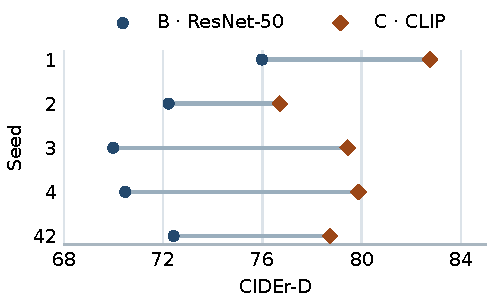
\includegraphics[width=\columnwidth]{figures/seed_comparison.pdf}
  \caption{CIDEr-D trên tập kiểm định theo năm seed trên Kaggle T4. Mỗi đường nối hai lượt chạy chung seed.}
  \label{fig:seeds}
\end{figure}

\begin{figure*}[t]
  \centering
  \begin{tabular}{@{}c@{\hspace{0.018\textwidth}}c@{\hspace{0.035\textwidth}}c@{\hspace{0.018\textwidth}}c@{}}
    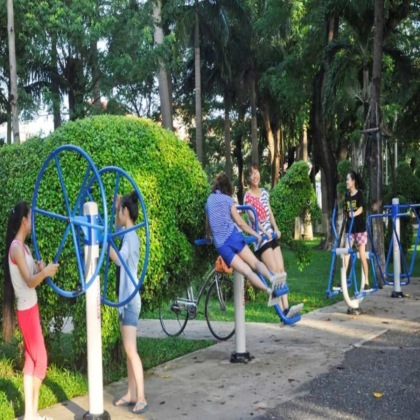
\includegraphics[width=.216\textwidth]{figures/scene_3091.jpg} &
    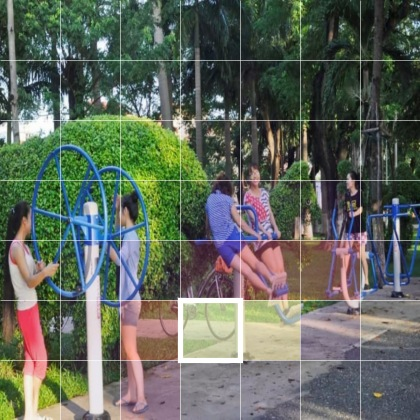
\includegraphics[width=.216\textwidth]{figures/attention_3091.jpg} &
    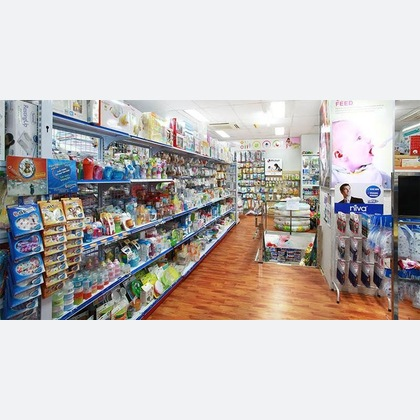
\includegraphics[width=.216\textwidth]{figures/scene_297.jpg} &
    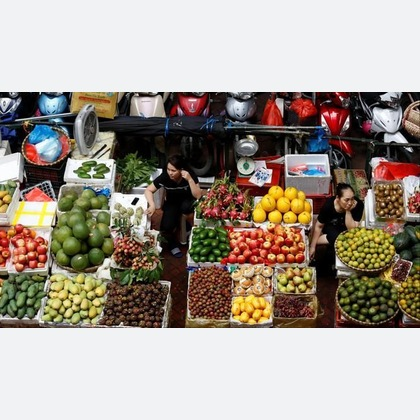
\includegraphics[width=.216\textwidth]{figures/scene_4568.jpg} \\
    \small (a) Ảnh 3091 &
    \small (b) Khi sinh “chụp” &
    \small (c) Ảnh đúng, hạng 392 &
    \small (d) Kết quả hạng 1
  \end{tabular}
  \caption{Ảnh test KTVIC và hai ca phân tích lỗi. (a--b) Ô viền trắng là vùng có trọng số cao nhất của A tại token “chụp”. (c--d) Hai kết quả từ chỉ mục B cho truy vấn về hàng hóa trên kệ: ảnh đúng có ID 297, còn ảnh 4568 đứng đầu.}
  \label{fig:cases}
\end{figure*}

\subsection{Lỗi chú thích và attention}

Tập phân tích có 40 ảnh test, ba cấu hình \modelA{}, \modelB{}, \modelAz{} và 120 câu. Hai lượt chấm xem 25 ảnh mỗi lượt, trong đó 10 ảnh trùng, với tên mô hình được ẩn. Mỗi câu nhận sáu cờ: sai vật thể, hành động, quan hệ, số lượng, chi tiết bịa hoặc lặp từ. Mỗi cờ có thể là $0$ (chưa thấy lỗi), $1$ (có lỗi) hoặc \texttt{?} (chưa rõ). Ở phần chung, 168/172 ô đã rõ trùng nhau trước khi đối chiếu (97,67\%). Tám ô còn lại chưa rõ ở cả hai lượt. Bốn bất đồng được rà lại dựa trên ảnh trước khi tổng hợp.

\begin{table}[t]
  \centering
  \begin{tabular}{lrrr}
    \toprule
    Loại lỗi & \modelA{} & \modelAz{} & \modelB{} \\
    \midrule
    Vật thể              & 7/37  & 9/36  & 10/38 \\
    Hành động            & 5/36  & 3/34  & 6/38 \\
    Quan hệ              & 2/38  & 2/39  & 7/38 \\
    Số lượng             & 0/40  & 1/40  & 0/40 \\
    Chi tiết bịa         & 11/40 & 8/40  & 6/39 \\
    Lặp từ               & 0/40  & 0/40  & 1/40 \\
    \midrule
    Có ít nhất một lỗi   & 20/34 & 23/33 & 24/34 \\
    \bottomrule
  \end{tabular}
  \caption{Số câu có lỗi trên số câu có nhãn đã rõ, tối đa 40 câu mỗi cấu hình. Hàng cuối tính là lỗi nếu có ít nhất một cờ 1, và chỉ tính là sạch nếu cả sáu cờ đều bằng 0.}
  \label{tab:errors}
\end{table}

Trong mẫu này, \modelB{} có nhiều câu sai quan hệ hơn \modelA{} (7/38 so với 2/38). \modelA{} lại có số câu bịa chi tiết cao nhất (11/40). Các cờ có thể đồng thời xuất hiện trên một câu, vì vậy tổng từng loại có thể lớn hơn số câu có lỗi. Bảng~\ref{tab:errors} mô tả mẫu đã xem, với quy trình chấm có AI hỗ trợ.

\subsection{Các ca minh họa}
\label{sec:cases}

\paragraph{Gọi sai hành động.}
Ảnh 3091 cho thấy một nhóm người dùng dụng cụ tập thể dục. \modelA{} sinh “có một nhóm người đang chụp ảnh tập thể dục ở trên đường”. \modelAz{} cũng sinh cụm “chụp ảnh”. Khi \modelA{} sinh “chụp”, ô gần bánh xe đạp và nền đường nhận trọng số cao nhất (11,05\%, hàng 6, cột 4 tính từ 1). A0 gán đều 2,04\% mỗi ô. Hình~\ref{fig:cases}a--b biểu diễn cách phân bố trọng số tại bước đó. Căn cứ để gán lỗi là nội dung câu và ảnh.

\paragraph{Tìm sai khi câu sinh thiếu từ khóa.}
Truy vấn “có nhiều loại hàng hoá được bày ra trên các kệ hàng” có đáp án ID 297. \modelB{} sinh “có một vài người đang đứng ở bên trong siêu thị”, nên câu sinh của ảnh đúng chỉ chia sẻ token “có” với truy vấn và đạt cosine 0,0134. Câu sinh của ảnh 4568 nói quả được bày trên kệ hàng và đạt 0,6941. Riêng “kệ” và “hàng” đóng góp khoảng 0,1997 vào điểm của ảnh đứng đầu. Hình~\ref{fig:cases}c--d minh họa sự khác biệt giữa nội dung ảnh và tín hiệu dùng để xếp hạng.

\paragraph{Tìm đúng và trường hợp hòa điểm.}
Với câu “đây là một bức ảnh chụp một tấm bản đồ”, chỉ mục \modelA{} trả đúng ảnh 5546 ở hạng 1 vì câu sinh giữ cụm “tấm bản đồ”. Với truy vấn về hàng hóa trên kệ, có bảy ảnh cùng chú thích và cùng cosine 0,8789 trong chỉ mục \modelA{}. Ảnh gốc 8678 đứng hạng 7 theo ID. Trong nhóm hòa điểm có những ảnh khác cũng phù hợp với mô tả.

\subsection{Điểm chú thích và điểm tìm ảnh}

Theo Bảng~\ref{tab:test}, \modelA{} tìm đúng 360/2.790 truy vấn ở top 5, so với 286 của \modelB{}. Chênh lệch là 2,65 điểm phần trăm (khoảng tin cậy 95\% từ 0,25 đến 4,84). \modelAz{} đạt 369 lượt, cao hơn \modelA{} chín lượt. Khoảng tin cậy 95\% của chênh lệch \modelAz{} trừ \modelA{} là từ $-1{,}97$ đến $2{,}62$ điểm phần trăm. \modelC{} có hạng trung vị tốt nhất (68), nhưng 308 lượt trúng top 5, thấp hơn cả hai cấu hình LSTM. BLEU và CIDEr-D đo độ khớp giữa câu sinh và tham chiếu cùng ảnh. Recall còn phụ thuộc liệu những từ khớp có giúp phân biệt ảnh gốc với các ảnh khác trong kho hay không.

\section{Kết luận}

Trên 558 ảnh test, LSTM có attention đạt 78,67 CIDEr-D và Transformer dùng CLIP đạt BLEU-4 cao nhất (30,51). LSTM attention đều đạt 13,23\% Recall@5, hơn LSTM attention học được chín truy vấn. Từ khóa bị bỏ sót và chú thích trùng làm nhiều ảnh khó phân biệt khi xếp hạng. Các thử nghiệm tiếp theo nên lặp đối chứng A/B và A/A0 qua nhiều seed, đồng thời chấm tìm ảnh trên truy vấn mới với nhiều ảnh phù hợp cho mỗi câu.

\section*{Khai báo sử dụng AI}

Codex hỗ trợ chuẩn bị mã, rà kết quả, chấm một lượt phiếu lỗi, soạn và biên tập LaTeX, vẽ sơ đồ và biểu đồ. Claude Code hỗ trợ phiếu do Phạm Thị Khánh Linh chấm và xem lại theo hồ sơ. Điểm, chú thích tự sinh và số đo huấn luyện trong bài lấy từ tệp thí nghiệm.

% Mốc cuối nội dung tính vào giới hạn tám trang theo đề. Các mục sau được miễn.
\raggedbottom
\section*{Hạn chế}

KTVIC chỉ đại diện cho miền ảnh đã thu thập. Tách theo âm tiết có thể chia một từ tiếng Việt thành nhiều đơn vị và làm thay đổi cách tính $n$-gram. Kết quả test dựa trên một seed và một checkpoint mỗi mô hình. Năm cặp B/C dùng cùng tập kiểm định, nên chúng cho thấy dao động theo seed trên tập đó. So sánh encoder thay đồng thời quy trình xử lý ảnh, kiến trúc, nguồn tiền huấn luyện và số chiều đặc trưng.

BLEU và CIDEr-D nhạy với từ ngữ trong năm câu tham chiếu, kể cả khi một câu khác diễn đạt đúng ảnh. Mẫu chấm lỗi chỉ gồm 40 ảnh và ba mô hình. Mức trùng nhãn đến từ hai lượt chấm có hỗ trợ AI. Bản đồ attention thể hiện trọng số nội bộ tại một bước sinh, chưa đủ để xác lập quan hệ nhân quả giữa vùng ảnh và token.

Đánh giá tìm ảnh dùng câu tham chiếu sẵn có và một ID đúng cho mỗi truy vấn. Người dùng có thể đặt câu khác cách diễn đạt trong tập, hoặc thấy nhiều ảnh đều phù hợp. Chỉ mục dựa vào một câu mỗi ảnh nên nhạy với chi tiết bị bỏ qua và với hòa điểm. Thời gian giải mã đo từ cache, chưa bao gồm trích đặc trưng cho ảnh mới hoặc thời gian truy vấn.

\section*{Đóng góp của thành viên}

\textbf{Lê Vân Anh (50\%).} Chuẩn bị và chia dữ liệu, cài đặt LSTM attention và đối chứng attention đều, xây vòng huấn luyện và tìm ảnh TF-IDF, đối chiếu kết quả tìm ảnh.

\textbf{Phạm Thị Khánh Linh (50\%).} Triển khai trích đặc trưng ResNet-50 và bộ chấm BLEU/CIDEr-D, cài Transformer, ghép encoder CLIP, huấn luyện đối chứng B/C và đối chiếu bảng kết quả test.

Cả hai thành viên tham gia phân tích lỗi và chuẩn bị nội dung báo cáo.

\bibliography{references}

\end{document}
